\section{Hardware Interface Between Microcontroller and Computer}\label{sec:hardware-interface-between-mcu-and-computer}

	\subsection{USB and UART}\label{ssec:usb-and-uart}
		Nowadays most computers do not have a serial port connector \cite{serialPortNeverSayDie}, the majority of communications with peripherals are done through USB ports. The choosen microcontroller for this project (as discussed on Section \ref{sec:mcu-hw}) does not have USB interface, only UART. 

		As it was explained in Section \ref{sssec:usb}, USB communication protocol is half-duplex, UART protocol is full-duplex though. While USB is composed of a differential pair of data wires, UART has one wire for receiving and another one for transmitting information. 

		In order to make this project compatible with most of modern computers, there is the need to have a USB to UART converter circuit.

	\subsection{Conversion Circuit}\label{ssec:usb-uart-conversion-circuit}

		The issue discussed in the previous section is not a new thing, so there are loads of integrated solutions to solve this issue \cite{usbSerialAdapter}. The choosen one was the Microchip's MCP2221A \cite{mcp2221a-datasheet}, this is a USB to UART/I$^2$C converter chip, it emulates a virtual serial port on the computer, making it possible to communicate with the microcontroller UART ports just using a pair of capacitors and a resistor as Figure \ref{fig:mcp2221a-basic-circuit} shows.

		\begin{figure}[htbp]
			\centering
				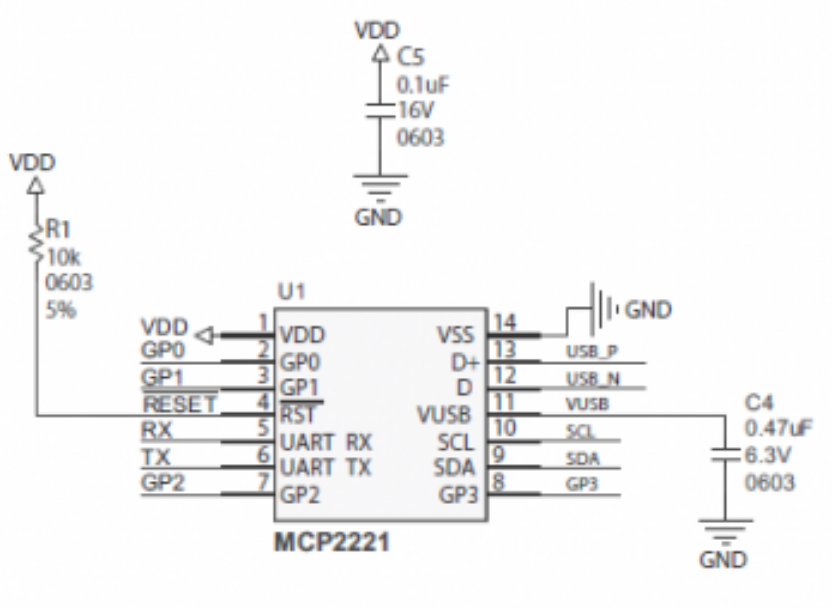
\includegraphics[scale=1.2]{figuras/fig-mcp2221a-basic-circuit}
			\caption{MCP2221A basic circuit \cite{mcp2221a-basic-circuit}}
			\label{fig:mcp2221a-basic-circuit}
		\end{figure}

		This chip already contains a internal 3V3 LDO in order to convert the 5V TTL level to the 3V3 standard level for USB data lines. The voltage supply for this IC is being supplied by the voltage from the USB cable because there is no need to keep this IC turned on when the USB cable is not connected.


	\subsection{Circuit Protection}\label{ssec:usb-uart-circuit-protection}
		In order to ensure reliability on the circuit, ESD protection is needed, every connection between the circuit board and the outside world has the potential to pick unwanted noise and ESD, and USB is not exclued from that problem \cite{circuit-protection-usb}.

		High-frequency noise could be filtered using low pass filters in both data lines using discrete passive components. Moreover, the data lines could be protected from ESD using discrete TVS. The number of discrete componentes needed to filter and protect the lines makes a discrete-component-solution unpractical, expensive and spacious. Nowadays there are unexpensive integrated solutions in order to save space on the PCB, one of them is the ON Semiconductor STF202-22T1G. This IC is a USB Filter with ESD protection, as the datasheet \cite{stf202-22t1g-datasheet} says: \textit{"This device is designed for applications requireing Line Termination, EMI filtering and ESD protection"}, making it more than ideal for this project. The STF202-22T1G internal circuit can be seen on Figure \ref{fig:stf202-22t1g-sch}.

		\begin{figure}[htbp]
			\centering
				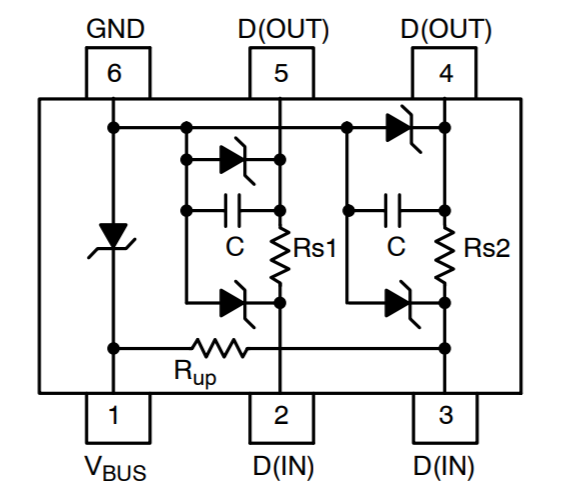
\includegraphics[scale=1.2]{figuras/fig-stf202-22t1g-sch}
			\caption{STF202-22T1G Internal Circuit \cite{stf202-22t1g-sch}}
			\label{fig:stf202-22t1g-sch}
		\end{figure}

	\subsection{Complete Circuit}\label{ssec:usb-uart-complete-circuit}

		For the final circuit the STF202-22T1G was connected before the MCP2221A in order to protect and filter the data lines. Moreover, two external resistors were added to the serial communication lines (based on the Arduino Rev3 Schematic \cite{arduino-rev3-schematic}). Figure \ref{fig:usb-uart-circuit} contains the final circuit.

		\begin{figure}[htbp]
			\centering
				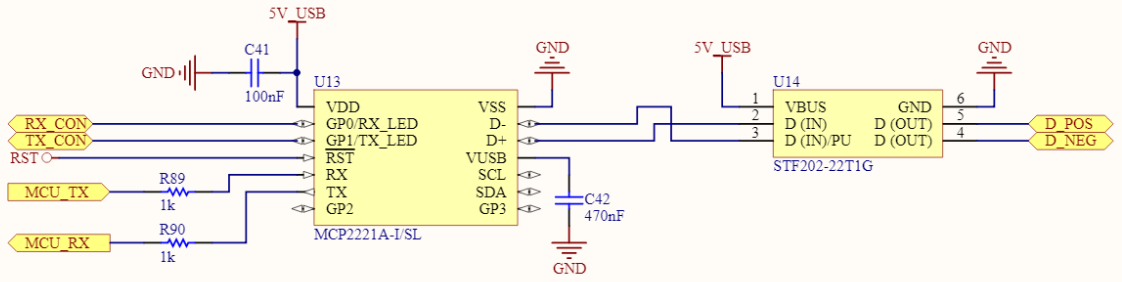
\includegraphics[scale=0.5]{figuras/fig-usb-uart-circuit}
			\caption{USB/UART Converter Circuit \cite{usb-uart-circuit}}
			\label{fig:usb-uart-circuit}
		\end{figure}

		The \textit{TX CON} and \textit{RX CON} lines are used in other to indicate when the MCP2221A chip is repectively transmitting or receiving data. This lines drain current when data is transmitted or received and are used to blink LEDs in other parts of the circuit board. 

		Both capacitors are decoupling capacitors for the 5V and 3V3 lines. 